\documentclass[conference]{IEEEtran}
\IEEEoverridecommandlockouts
% The preceding line is only needed to identify funding in the first footnote. If that is unneeded, please comment it out.
\usepackage{cite}
\usepackage{amsmath,amssymb,amsfonts}
\usepackage{algorithmic}
\usepackage{graphicx}
\usepackage{textcomp}
\usepackage{xcolor}
\usepackage{booktabs}
\usepackage{url}
\usepackage{tikz}
\usetikzlibrary{positioning,arrows.meta,shapes.geometric,fit,backgrounds}
\def\BibTeX{{\rm B\kern-.05em{\sc i\kern-.025em b}\kern-.08em
    T\kern-.1667em\lower.7ex\hbox{E}\kern-.125emX}}
\begin{document}

\title{Order-2 Co-occurrence TF-IDF for Interaction-Free Perfume Retrieval}

\author{\IEEEauthorblockN{Azam Azri}
\IEEEauthorblockA{\textit{Master's Program in Informatics} \\
\textit{Affiliation (to be completed)}\\
Yogyakarta, Indonesia \\
azamazriahmad@mail.ugm.ac.id}
}

\maketitle

\begin{abstract}
Content-based perfume recommenders rank products by order-one accord similarity, such as
cosine or Jaccard over note sets, and treat accords as independent. Whether modeling how
accords \emph{co-occur} improves recommendation has not been tested under a leakage-free
protocol. Most product catalogs also record no user interactions, which rules out the
collaborative and knowledge-graph recommenders that need an interaction signal. This paper
studies interaction-free, content-based perfume recommendation, cast as a retrieval task:
given a reference perfume, the catalog is ranked to surface the product that best matches
it, and a held-out inspired-by edge supplies ground-truth relevance. The proposed matcher
is parameter-free. It augments accord TF-IDF with accord-pair (order-two) tokens, its
cosine score splits additively into an order-one and an order-two term, and it emits
auditable co-occurrence paths for explanation. The evaluation covers 340 products and 209
reference perfumes under leave-one-out ranking, behind a three-source firewall whose query
accords are independently verified from Fragrantica. Across fifteen methods spanning
marginal similarity, neural embeddings, perceptual-taxonomy transport, and learned models,
the order-two matcher attains the best mean reciprocal rank (MRR 0.496) and exceeds the
TF-IDF baseline (0.454) by a modest but robust margin ($\Delta$MRR $+0.042$, 95\% CI
$[+0.019,+0.067]$, Wilcoxon $p=8.7\times10^{-8}$); order-two terms supply 81.3\% of the
top-ranked score.
\end{abstract}

\begin{IEEEkeywords}
recommender systems, content-based retrieval, co-occurrence, TF-IDF, explainability,
fragrance, non-circular evaluation
\end{IEEEkeywords}

\section{Introduction}
Choosing a perfume is hard. A shopper who likes an expensive branded scent often wants an
affordable local product that smells the same, and a content-based recommender can help.
Each perfume is described by a small set of olfactory \emph{accords}---for example
\textit{amber}, \textit{woody}, or \textit{warm spicy}---and two perfumes that share
accords tend to smell alike. Existing perfume recommenders rank products almost only by
order-one accord similarity: cosine over term frequency--inverse document frequency
(TF-IDF) vectors, or Jaccard over accord sets \cite{r23,r24,r28}. Such marginal
representations score each accord independently and ignore the structure in which accords
\emph{co-occur}.

A second constraint matters in practice. Many real catalogs store only content---accord
lists and family labels---and record no ratings or clicks. This rules out the
interaction-driven recommenders that dominate the higher-order and knowledge-graph
literature, such as collaborative filtering, LightGCN, KGIN, and KGAT \cite{r20}, because
they learn from a user--item signal the data does not contain. Methods that exploit item
co-occurrence and higher-order structure do report strong gains, but only in
interaction-based settings such as session or multi-behavior recommendation
\cite{r1,r2,r3,r4,r5}. Whether order-two accord co-occurrence helps in a purely
content-based, interaction-free setting---and whether it helps under an evaluation that
cannot leak the answer---is still open.

A third assumption is common in adjacent fields: that adding perceptual or learned
\emph{structure} improves retrieval. Odor science arranges accords on sensory wheels and
perceptual maps \cite{r10,r12,r13}, and much work assumes such geometry should help. Yet on
small, imbalanced datasets, simple baselines often match or beat flexible models that
overfit \cite{r14,r15,r16,r17}. This tension has not been examined for interaction-free
perfume recommendation.

This paper addresses these gaps with a deliberately simple, parameter-free method and a
non-circular protocol. Accords and accord-pairs---the nodes and edges of a co-occurrence
graph---are weighted by inverse document frequency and compared by cosine. The score splits
additively into an order-one (marginal) term and an order-two (co-occurrence) term, and the
shared accord-pairs become auditable explanation paths. The matcher carries no trained
parameters, because added capacity is shown to overfit. The contribution is therefore a
\emph{finding and a protocol}, not a new model, at a moderate applied scope.

The paper makes four contributions. \emph{Task and protocol.} It casts interaction-free,
content-based perfume recommendation as a retrieval task and defines a non-circular
evaluation with a three-source firewall: local item accords, externally sourced query
accords verified from Fragrantica, and held-out inspired-by labels (the imitation, or
``dupe,'' relation, used only as ground truth). It also makes explicit why interaction-based
recommenders (KGAT, LightGCN, KGIN) cannot be compared on this data. \emph{Method.} It
proposes an order-two co-occurrence TF-IDF matcher whose cosine score decomposes into
order-one and order-two terms and yields faithful-by-construction explanation paths.
\emph{Finding.} It gives a first non-circular demonstration that order-two co-occurrence
ranks first among fifteen methods, ahead of all twelve comparators across four
paradigms---marginal similarity, neural embeddings, perceptual-taxonomy transport, and
learned models---while neither proposed variant improves on it. Honest caveats accompany the
claim: the gain over the TF-IDF baseline is modest ($+0.042$ MRR) yet robust, the
Sentence-BERT loss is partly due to query--product text asymmetry, and the moderate learned
methods only match the baseline. \emph{Reproducibility.} It provides a complete,
deterministic benchmark of fifteen methods with paired significance tests and bootstrap
confidence intervals. The remainder of the paper reviews related work, formalizes the
problem, presents the method, describes the setup, and reports, discusses, and bounds the
results.

\section{Related Work}\label{sec:related}

\subsection{Content-based perfume recommendation}
Perfume recommenders are overwhelmingly content-based and order-one. Lutan \cite{r23}
surveys the field and identifies subjectivity and sparse sensory data as core obstacles;
Nurmuthia \textit{et al.} \cite{r24} rank perfumes by cosine and Jaccard similarity over
notes, and Fannisa \textit{et al.} \cite{r28} report that a TF-IDF content-based filter
outperforms a Word2Vec variant. These systems treat accords as independent terms; none
tests whether modeling accord \emph{co-occurrence} helps, and none does so under a
protocol that prevents the label from leaking into the features---exactly the gap this
work targets.

\subsection{Co-occurrence, higher-order, and explainable recommendation}
Outside fragrance, co-occurrence and higher-order structure reliably help: higher-order
graph neural networks \cite{r1}, item co-occurrence graphs for session-based
recommendation \cite{r2}, graph-based feature crossing \cite{r3}, multi-modal session
models \cite{r4}, and negative co-occurrence signals \cite{r5} all improve accuracy.
Crucially, every one consumes a user--item or session signal. Knowledge-graph and
path-based explainable recommenders---KGAT \cite{r20} and related reasoning models
\cite{r18,r19,r21}---likewise depend on interactions to learn embeddings and attention,
and their paths can be only loosely tied to the score. Because the catalog studied here
has no interactions, KGAT, LightGCN, and KGIN cannot be instantiated and are excluded from
comparison. The proposed method instead lifts co-occurrence into the content representation
itself and derives explanation paths directly from the shared accord-pairs that produce the
score, so they are discriminative (weighted by inverse document frequency) and faithful by
construction.

\subsection{Perceptual structure, transport, and simple baselines}
Olfactory science represents odors with sensory wheels and perceptual maps
\cite{r10,r11,r12,r13}, suggesting that imposing such geometry should aid retrieval, and
transport-based distances on trees and graphs offer a principled way to compare
distributions over it \cite{r7,r8,r9,r9b}. This hypothesis is operationalized here as a
tree-Wasserstein distance over the Edwards wheel and measured---rather than assumed. A
countervailing lesson is that flexible, high-capacity models fail to beat simple baselines
on scarce or imbalanced data: linear baselines remain competitive for gene-perturbation
prediction \cite{r14}, overfitting under class imbalance is well documented on small
datasets \cite{r15,r16,r17}, and cold-start recommenders lean on content rather than
capacity \cite{r25,r26,r27}. These motivate the parameter-free design adopted here. To the
best of current knowledge, the intersection studied---interaction-free, non-circular,
order-two co-occurrence for perfume recommendation, used to test the benefit of perceptual,
neural, and learned structure---is unaddressed by this literature.

\section{Problem Formulation}\label{sec:problem}

\subsection{Problem setup}
Let $\mathcal{P}=\{p_1,\dots,p_N\}$ be the catalog of local products, with $N=340$. Each
product $p$ carries a set of olfactory accords $A(p)\subseteq\mathcal{V}$ and a family
label, where $\mathcal{V}$ is the accord vocabulary. Let $\mathcal{Q}$ be the set of
reference perfumes (branded originals); each reference $q$ carries accords $A(q)$ and a
family. The imitation (``dupe'') relation gives, for each reference, a ground-truth set
\begin{equation}
g(q)=\{\,p\in\mathcal{P}\;:\;\textit{inspired\_by}(p)=q\,\}, \label{eq:gold}
\end{equation}
the products built to smell like $q$. A method scores every product, $s(q,p)$, and ranks
the whole catalog; quality is the rank of the ground-truth product, measured by the metrics
defined later. Of the $340$ products, $243$ carry a label and $97$ are unlabeled originals
kept in the pool as genuine distractors; $209$ references have at least one labeled product
and form the leave-one-out evaluation set. Local and reference vocabularies share $56$
accords.

The deployed recommender and the evaluation share an \emph{identical} scoring engine; they
differ only in the query source (free user text or a reference perfume) and in whether a
ground-truth answer exists. A reference perfume is never returned as output: the pool is the
local catalog.

\subsection{A non-circular firewall}
The central methodological risk is circularity: if the query features were copied from the
very products they are meant to retrieve, any accord overlap would be a tautology. A
three-source separation guards against this (Table~\ref{tab:firewall}). Query accords are
sourced independently from Fragrantica---$264$ of $266$ \texttt{source\_url} entries resolve
to perfume-specific Fragrantica pages---rather than back-filled from the local catalog, so
the benchmark is non-circular by construction.

\begin{table}[htbp]
\caption{Three-source firewall for non-circular evaluation}
\begin{center}
\begin{tabular}{lll}
\toprule
\textbf{Component} & \textbf{Source} & \textbf{Independent of} \\
\midrule
Item features  & local catalog accords        & the label \\
Query features & Fragrantica accords (external) & local catalog \& label \\
Label          & held-out \textit{inspired\_by} edge & accord similarity \\
\bottomrule
\end{tabular}
\label{tab:firewall}
\end{center}
\end{table}

A leakage audit further removes identity-bearing text before any text-based method sees it:
the \texttt{interpreted\_as} field equals the reference perfume name and is never exposed,
and a distinctive token of a product's own reference name appears in the free-text
\texttt{meaning} of $32$ of $340$ products; these tokens are stripped prior to embedding.

\subsection{Scope and validity}
Collaborative and knowledge-graph recommenders---LightGCN, KGIN, and KGAT \cite{r20}---take
a user--item interaction matrix $R\in\{0,1\}^{U\times I}$ and learn embeddings from it. The
catalog studied here has no users ($U=\varnothing$), so $R$ is undefined and these models
cannot be instantiated; the exclusion is a property of the data and is stated explicitly
rather than papered over with vacuous numbers. A second caveat concerns the proxy itself:
the imitation relation measures \emph{perceptual} match, not user satisfaction. Because an
imitation is built to smell like its target, query--target accord overlap is high (about
$86\%$ of a target's accords appear in the query). This overlap is a genuine signal rather
than an artifact, and it bounds how much any method can improve over the marginal baseline.

\section{Proposed Method}\label{sec:method}
The proposed matcher represents each fragrance not only by which accords it contains
but by which accords \emph{co-occur} in it, weights both by rarity, and compares two
fragrances by a single cosine that splits cleanly into a marginal term and a
co-occurrence term. It has no trained parameters. Fig.~\ref{fig:concept} illustrates the
core idea, and Fig.~\ref{fig:arch} summarizes the pipeline.

\begin{figure}[t]
\centering
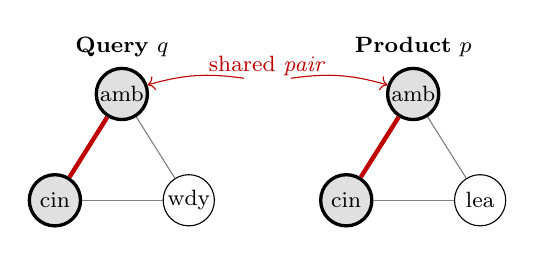
\begin{tikzpicture}[
  font=\footnotesize,
  acc/.style={draw, circle, minimum size=6.5mm, inner sep=0pt, fill=white},
  sh/.style={draw, circle, minimum size=6.5mm, inner sep=0pt, fill=black!12, very thick},
  e1/.style={gray},
  e2/.style={ultra thick, red!75!black}]
% Query triangle (left)
\node at (0,1.95) {\textbf{Query} $q$};
\node[sh] (qa) at (0,1.35) {amb};
\node[sh] (qc) at (-0.85,0) {cin};
\node[acc] (qw) at (0.85,0) {wdy};
\draw[e1] (qa)--(qw); \draw[e1] (qc)--(qw);
\draw[e2] (qa)--(qc);
% Product triangle (right)
\node at (3.7,1.95) {\textbf{Product} $p$};
\node[sh] (pa) at (3.7,1.35) {amb};
\node[sh] (pc) at (2.85,0) {cin};
\node[acc] (pl) at (4.55,0) {lea};
\draw[e1] (pa)--(pl); \draw[e1] (pc)--(pl);
\draw[e2] (pa)--(pc);
\node[red!75!black] at (1.85,1.7) {\footnotesize shared \emph{pair}};
\draw[->,red!75!black] (1.55,1.55) to[bend right=12] (qa);
\draw[->,red!75!black] (2.15,1.55) to[bend left=12] (pa);
\end{tikzpicture}
\caption{Order-1 versus order-2 matching. Shaded nodes are accords shared by reference $q$
and candidate product $p$ (order-1). The bold red edge is a rare accord \emph{pair}
(\textit{amber--cinnamon}) that co-occurs in both (order-2). A distractor may share the same
individual accords yet lack this signature pairing; the shared rare pair, not the shared
accords, lifts the true match to the top.}
\label{fig:concept}
\end{figure}

\subsection{Co-occurrence representation}
For a fragrance $f$ with accord set $A(f)$, define its accord co-occurrence graph
$G_f=(A(f),E_f)$ whose edges are the unordered accord pairs
\begin{equation}
E_f=\{(a,b)\;:\;a,b\in A(f),\ a<b\}. \label{eq:edges}
\end{equation}
The token set of $f$ is the union of its accords (unigrams) and its accord pairs
(bigrams),
\begin{equation}
T(f)=A(f)\,\cup\,E_f. \label{eq:tokens}
\end{equation}

\subsection{Rarity weighting and normalization}
Tokens are weighted by inverse document frequency over the catalog of $N$ products.
With document frequency $\mathrm{df}(t)=\lvert\{f:t\in T(f)\}\rvert$,
\begin{equation}
\mathrm{idf}(t)=\log\!\frac{1+N}{1+\mathrm{df}(t)}+1. \label{eq:idf}
\end{equation}
Rare signature pairs receive a high weight, whereas ubiquitous hub accords (e.g.,
\textit{woody}, \textit{citrus}) receive a low weight; the hub penalty is therefore
automatic and parameter-free. Each fragrance becomes a sparse vector
\begin{equation}
v_f[t]=
\begin{cases}
\mathrm{idf}(t) & \text{if } t\in T(f),\\
0 & \text{otherwise,}
\end{cases}
\label{eq:vector}
\end{equation}
which is then $L_2$-normalized, $v_f\leftarrow v_f/\lVert v_f\rVert_2$.

\subsection{Similarity and additive decomposition}
The score between a query $q$ and a product $p$ is the cosine of their token vectors,
which separates exactly into an order-one (marginal) and an order-two (co-occurrence)
contribution:
\begin{equation}
s(q,p)=\frac{S_1(q,p)+S_2(q,p)}{\lVert v_q\rVert\,\lVert v_p\rVert}, \label{eq:score}
\end{equation}
\begin{align}
S_1(q,p)&=\sum_{a\in A(q)\cap A(p)}\mathrm{idf}(a)^2,\label{eq:s1}\\
S_2(q,p)&=\sum_{e\in E_q\cap E_p}\mathrm{idf}(e)^2.\label{eq:terms}
\end{align}
Here $S_1$ rewards shared accords and $S_2$ rewards shared accord \emph{pairs}; because
both blocks share one normalizer, the two terms add up to the full score. Empirically,
the order-two term $S_2$ accounts for $81.3\%$ of the top-ranked score, confirming that
co-occurrence, not marginal overlap, drives retrieval. Ranking the $340$ products by
$s(q,p)$ in descending order and taking the three highest yields the Top-3 output.

\subsection{Explanation paths}
Because the score is a sum over shared tokens, every recommendation is explained by the
same quantities that produced it. For each Top-3 product, the shared accord pairs
$E_q\cap E_p$ are emitted as co-occurrence \emph{paths}, each carrying its weight
$\mathrm{idf}(e)^2$ and the Edwards fragrance-wheel super-family \cite{r10} of its two
accords (or \textit{cross-family} when they differ); shared single accords are emitted
as node paths. The resulting \texttt{kg\_paths} are auditable and faithful by
construction---they are not a post-hoc rationalization but the score decomposition
itself---and serve a downstream explainability layer.

\begin{figure}[t]
\centering
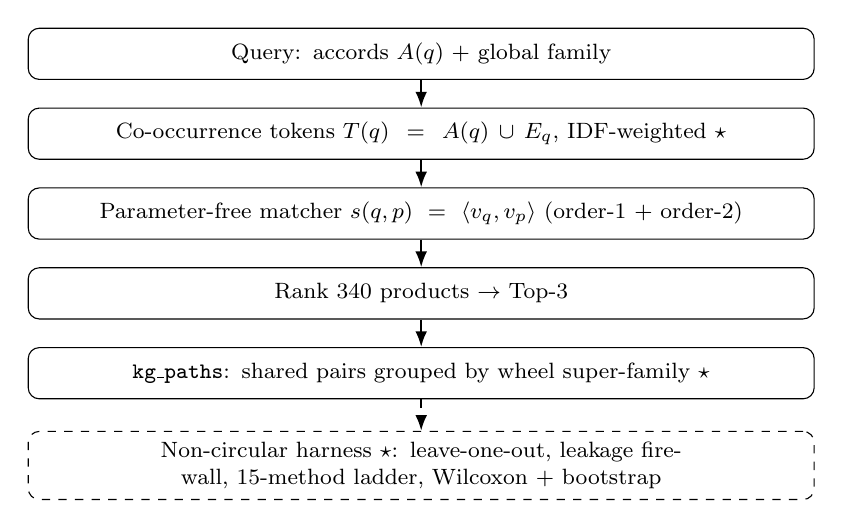
\begin{tikzpicture}[
  font=\footnotesize,
  box/.style={draw, rounded corners, align=center, text width=0.80\linewidth,
              inner sep=4pt, minimum height=6.5mm},
  hbox/.style={draw, dashed, rounded corners, align=center, text width=0.80\linewidth,
               inner sep=4pt},
  arr/.style={-{Latex[length=2mm]}, thick}]
\node[box] (q) {Query: accords $A(q)$ + global family};
\node[box, below=3.5mm of q] (g) {Co-occurrence tokens $T(q)=A(q)\cup E_q$, IDF-weighted~$\star$};
\node[box, below=3.5mm of g] (m) {Parameter-free matcher $s(q,p)=\langle v_q,v_p\rangle$ (order-1 $+$ order-2)};
\node[box, below=3.5mm of m] (r) {Rank 340 products $\rightarrow$ Top-3};
\node[box, below=3.5mm of r] (k) {\texttt{kg\_paths}: shared pairs grouped by wheel super-family~$\star$};
\draw[arr] (q)--(g); \draw[arr] (g)--(m); \draw[arr] (m)--(r); \draw[arr] (r)--(k);
\node[hbox, below=4mm of k] (h) {Non-circular harness~$\star$: leave-one-out, leakage firewall, 15-method ladder, Wilcoxon + bootstrap};
\draw[arr, dashed] (k)--(h);
\end{tikzpicture}
\caption{Framework overview. A query is turned into an IDF-weighted co-occurrence token
vector, matched against the $340$ products by a parameter-free cosine, and the Top-3 are
returned with auditable \texttt{kg\_paths}. The whole pipeline is evaluated by a
non-circular harness. $\star$ marks the three novelty points.}
\label{fig:arch}
\end{figure}

\subsection{Design rationale}
The matcher is deliberately parameter-free. On a catalog this sparse---$209$ queries,
one relevant product each---added capacity overfits, as the experiments confirm: a
learning-to-rank fusion does not significantly beat the bare cosine, and high-dimensional
learned variants collapse, as reported in the results. Simplicity is thus a design
decision grounded in the data regime, not an omission.

\section{Experimental Setup}\label{sec:setup}

\subsection{Dataset and provenance}
The catalog contains $340$ local products; $243$ carry an imitation label and $97$ are
unlabeled originals retained as distractors. After joining each labeled product to its
reference perfume, $209$ references have at least one labeled product and form the
leave-one-out evaluation set. Local and reference vocabularies share $56$ accords, drawn
from $17$ local and $49$ reference families. Accord lists are parsed by splitting on commas
and semicolons, lower-casing, and trimming. Crucially, query accords are taken from the
reference table whose entries are independently sourced: $264$ of $266$ \texttt{source\_url}
values resolve to perfume-specific Fragrantica pages, so query features are not back-filled
from the catalog they retrieve.

\subsection{Methods}
Fifteen methods (Table~\ref{tab:results}) are evaluated in three tiers. Tier~1 is
established baselines: marginal accord similarity (Jaccard, TF-IDF cosine, BM25) and neural
embeddings (multilingual Sentence-BERT \cite{r22} over the textual fields, Word2Vec over
accord sequences, node2vec over the co-occurrence graph). Tier~2 is structured or learned
comparators that test whether added structure helps: a tree-Wasserstein distance over the
Edwards wheel \cite{r10}, a positive pointwise mutual information (PPMI) embedding with
truncated SVD, a signature-subgraph learning-to-rank model, a per-bigram salience logistic
model, a low-rank bilinear metric, and a gradient-boosting fusion. Tier~3 is the proposed
family: the order-two matcher (P1), a learning-to-rank fusion (P2), and a hub-discriminative
IDF ablation (P3). B2 (TF-IDF cosine) is the primary marginal baseline.

\subsection{Metrics}
With one relevant product per query, the metrics are mean reciprocal rank (MRR) and Hits@$k$,
\begin{align}
\mathrm{MRR}&=\frac{1}{|\mathcal{Q}|}\sum_{q\in\mathcal{Q}}\frac{1}{r_q},\label{eq:mrr}\\
\mathrm{Hits}@k&=\frac{1}{|\mathcal{Q}|}\sum_{q\in\mathcal{Q}}\mathbf{1}[\,r_q\le k\,],\label{eq:hits}
\end{align}
where $r_q$ is the rank of the best (smallest-rank) ground-truth product for query $q$, and
$k\in\{1,3\}$. Ties in score are resolved by the expected reciprocal rank under uniform
random tie-breaking, which neither rewards nor penalizes tie-heavy methods.

\subsection{Protocol and significance}
Every method ranks the full pool of $340$ products. Supervised methods (A3--A6, P2) are
scored out-of-fold with $5$-fold \emph{GroupKFold} grouped by query, so no query appears
in both training and test. Deterministic methods are run once; stochastic methods (A2,
A5, B5, B6, and the fold-shuffled learning-to-rank models) are run over $5$ seeds and
reported as mean$\pm$standard deviation. Statistical significance against the proposed
method uses the Wilcoxon signed-rank test paired across queries on the reciprocal ranks;
because deterministic methods have no seed variance, significance is computed across
queries rather than across seeds. Confidence intervals for the difference in MRR use
$10{,}000$ bootstrap resamples over queries. For the text-based method, the leakage audit
of Section~\ref{sec:problem} is applied before embedding. The pipeline is implemented in
Python with fixed seeds for full reproducibility; only the optional Sentence-BERT baseline
requires a pretrained model download.

\section{Results}\label{sec:results}

\subsection{Retrieval accuracy}
Table~\ref{tab:results} reports MRR, Hits@1, and Hits@3 for all fifteen methods. The
proposed order-two matcher P1 reaches MRR $0.496$, the top score among the twelve
comparison methods; the next best comparator, the gradient-boosting fusion A6, trails at
$0.457$, and the primary TF-IDF baseline B2 at $0.454$. The learning-to-rank fusion P2 is
numerically marginally higher ($0.500$) but, as shown below, is statistically
indistinguishable from P1; the parameter-free P1 is therefore the method of
record and P2 an ablation. The remaining paradigms fall clearly behind: neural
embeddings (B6 $0.340$, B4 $0.272$, B5 $0.185$), the perceptual-taxonomy transport (A1
$0.284$), and the high-dimensional learned models (A5 $0.150$, A4 $0.139$) are all well
below the marginal baseline, while the moderate learned models (A2 $0.444$, A6 $0.457$)
only reach it.

\begin{table*}[t]
\caption{Methods, retrieval accuracy, and significance against the proposed P1. $\Delta$MRR
and Wilcoxon $p$ compare P1 with each method, paired across queries (95\% bootstrap
confidence intervals given in the text). Stochastic methods are averaged over 5 seeds; best
in bold.}
\begin{center}
\begin{tabular}{llccccc}
\toprule
\textbf{ID} & \textbf{Method (paradigm)} & \textbf{MRR} & \textbf{H@1} & \textbf{H@3} & \textbf{$\Delta$MRR vs.\ P1} & \textbf{Wilcoxon $p$} \\
\midrule
\textbf{P1} & order-2 co-occ.\ TF-IDF \textit{(proposed)} & \textbf{0.496} & \textbf{0.378} & \textbf{0.562} & --- & --- \\
P2 & P1 $+$ LTR fusion & 0.500 & 0.379 & 0.580 & $-0.005$ & $0.18$ (n.s.) \\
P3 & P1 $+$ hub-discriminative IDF & 0.448 & 0.335 & 0.491 & $+0.049$ & $6.2\times10^{-10}$ \\
\midrule
B1 & Jaccard (marginal) & 0.428 & 0.303 & 0.487 & $+0.069$ & $6.6\times10^{-3}$ \\
B2 & TF-IDF cosine (baseline) & 0.454 & 0.335 & 0.507 & $+0.042$ & $8.7\times10^{-8}$ \\
B3 & BM25 (marginal) & 0.388 & 0.278 & 0.433 & $+0.108$ & $8.3\times10^{-12}$ \\
B4 & Sentence-BERT (neural) & 0.272 & 0.163 & 0.311 & $+0.225$ & $1.6\times10^{-11}$ \\
B5 & Word2Vec (neural) & 0.185 & 0.110 & 0.182 & $+0.294$ & $2.0\times10^{-16}$ \\
B6 & node2vec (neural) & 0.340 & 0.233 & 0.371 & $+0.181$ & $2.7\times10^{-11}$ \\
A1 & wheel tree-Wasserstein (perceptual) & 0.284 & 0.174 & 0.306 & $+0.213$ & $3.9\times10^{-13}$ \\
A2 & PPMI $+$ SVD (learned) & 0.444 & 0.343 & 0.498 & $+0.054$ & $3.9\times10^{-3}$ \\
A3 & signature LTR (learned) & 0.433 & 0.303 & 0.500 & $+0.066$ & $5.7\times10^{-8}$ \\
A4 & bigram salience (learned) & 0.139 & 0.060 & 0.145 & $+0.367$ & $2.7\times10^{-21}$ \\
A5 & bilinear metric (learned) & 0.150 & 0.072 & 0.150 & $+0.332$ & $2.5\times10^{-21}$ \\
A6 & GBM fusion (learned) & 0.457 & 0.325 & 0.533 & $+0.052$ & $2.3\times10^{-2}$ \\
\bottomrule
\end{tabular}
\label{tab:results}
\end{center}
\end{table*}

\subsection{Significance}
The last two columns of Table~\ref{tab:results} pair P1 against every other method across
queries. P1 has a
positive, significant advantage over all twelve comparators. The headline comparison
against the marginal baseline B2 is modest but robust: $\Delta\mathrm{MRR}=+0.042$, with a
$95\%$ bootstrap confidence interval of $[+0.019,+0.067]$ and Wilcoxon
$p=8.7\times10^{-8}$. Margins are far larger over the neural and high-dimensional learned
methods (e.g., $+0.225$ over B4, $+0.294$ over B5, $+0.367$ over A4). Against the moderate
learned models the gain is small yet still significant ($+0.054$ over A2, $+0.052$ over
A6), so they match, not surpass, the baseline rather than failing outright. The fusion
variant P2 does not significantly differ from P1
($\Delta\mathrm{MRR}=-0.005$, $p=0.18$), confirming that added learning capacity is
unnecessary.

\subsection{Where the signal comes from}
Decomposing the P1 score by~\eqref{eq:score}--\eqref{eq:terms} shows that the order-two
term $S_2$ contributes, on average, $81.3\%$ of the top-ranked score, against $18.7\%$ for
the order-one term $S_1$. The advantage of P1 is therefore not a re-weighting of marginal
similarity but a genuinely second-order effect: shared rare accord \emph{pairs}, not
shared individual accords, separate the correct product from the distractors.

\section{Discussion}\label{sec:discussion}

\subsection{RQ1: order-two versus marginal similarity}
Order-two co-occurrence beats the marginal baseline, but modestly. P1 ranks first among
all twelve comparison methods and improves on B2 by $\Delta\mathrm{MRR}=+0.042$, an effect
small in absolute terms yet robust: the $95\%$ bootstrap interval $[+0.019,+0.067]$
excludes zero and the paired Wilcoxon test is decisive ($p=8.7\times10^{-8}$). That the
small headline gain is a genuine second-order effect, not noise, follows from the
decomposition: order-two terms supply $81.3\%$ of the top-ranked score, so shared rare
accord \emph{pairs}---not individual accords---lift the correct product. The gain cannot be
large by construction (Section~\ref{sec:problem}): with about $86\%$ of a target's accords
already in the query, the marginal baseline starts from a high floor. Order-two structure
thus helps reliably, not dramatically.

\subsection{RQ2: does added structure help?}
No comparator surpasses the simple matcher, but they fail at two magnitudes that should
not be conflated. The perceptual transport A1 ($0.284$), neural embeddings B4 ($0.272$),
B5 ($0.185$), B6 ($0.340$), and high-dimensional learned models A4 ($0.139$), A5 ($0.150$)
fall well below even the marginal baseline (gaps to P1 up to $+0.367$, $p<10^{-16}$). They
share one failure mode: each smooths or re-embeds the discrete accord-pair signal into a
continuous space, erasing the rare, discriminative co-occurrences that the exact-match
cosine preserves, and the high-capacity learned models additionally overfit the severe
one-positive-per-query imbalance. The claim must be softened, however, for the two moderate
learned methods: PPMI+SVD (A2, $0.444$) and GBM fusion (A6, $0.457$) land essentially on
the baseline B2 ($0.454$); P1 still beats them significantly ($+0.054$, $+0.052$), so they
\emph{match} the baseline without surpassing it rather than fail outright. The weak
Sentence-BERT result is likewise only partial evidence against neural semantics: query and
product text are asymmetric by construction---sparse accord lists against rich Indonesian
prose---so B4 is penalized by a text-distribution mismatch independent of its semantic
quality, which stops short of showing that neural semantics cannot help under a more
symmetric text regime.

\subsection{Why the simplest method wins, and what it explains}
That the most capable comparators lose while the parameter-free P1 wins matches a recurring
lesson on small, imbalanced data \cite{r14,r15,r16,r17}, and two internal controls confirm
it: the learning-to-rank fusion P2 ($0.500$) is statistically indistinguishable from the
bare cosine ($\Delta\mathrm{MRR}=-0.005$, $p=0.18$), so trained weights buy nothing, and
the learned variants A4/A5 collapse to the bottom of the table---the signature of
overfitting. Simplicity is therefore a design choice grounded in the data regime, not an
omission. The same design yields explanations for free: because the score is a sum over
shared tokens, each Top-3 product exports \texttt{kg\_paths}---the shared accord-pairs
$E_q\cap E_p$ with weight $\mathrm{idf}(e)^2$ and Edwards-wheel super-family---that are
faithful by construction rather than post-hoc. For the query \textit{1~Million}, for
instance, the ground-truth product is supported by signature pairs such as
\textit{amber--cinnamon} and \textit{cinnamon--warm spicy}. A counterfactual edge-ablation study quantifying their
faithfulness beyond the order-one/order-two decomposition is left to a downstream
explainability collaboration.

\subsection{Threats to validity}
Several limitations bound how strongly the result should be read. Accords are binary:
the catalog records no per-accord intensity, so products with identical accord sets are
indistinguishable and an intensity-weighted representation cannot be tested. The evaluation
set is small---$209$ queries, one relevant product each---so statistical power is bounded
(hence the reported intervals and paired tests) and the headline effect is correspondingly
modest. The imitation relation is a \emph{perceptual} proxy, not user satisfaction, and its
high query--target overlap is intrinsic to the task. The contribution is scoped to a finding
and a protocol, not a model: the matcher is parameter-free by design and offers no
mechanism to exploit richer signals (intensity, symmetric text, interactions) should they
appear. Finally, all results come from a single proprietary catalog in one fragrance
market, so external validity to other catalogs, domains, or larger vocabularies is untested
and should not be assumed.

\section{Conclusion}\label{sec:conclusion}
This work studied interaction-free, content-based perfume recommendation and asked whether
modeling the co-occurrence of accords improves retrieval over the marginal similarity that
dominates the field. The contribution is a finding and a protocol rather than a new model.
The task is formalized as a retrieval problem behind a non-circular evaluation---a
three-source firewall with externally verified query accords, a leakage audit, and a
fifteen-method comparison ladder---and the reason interaction-driven recommenders such as
KGAT, LightGCN, and KGIN cannot be instantiated on a catalog with no user interactions is
made explicit. Within this protocol, a deliberately parameter-free matcher that
augments accord TF-IDF with order-two accord-pair tokens ranks first among all fifteen
methods, beating every comparator across four paradigms---marginal similarity, neural
embeddings, perceptual-taxonomy transport, and learned models.

The result is reported with its caveats intact: the gain over the baseline is modest
($\Delta\mathrm{MRR}=+0.042$) yet robust and significant ($p=8.7\times10^{-8}$), with
$81.3\%$ of the top-ranked score from the order-two term; moderate learned methods match
rather than fall below the baseline; the Sentence-BERT result is partly a text-asymmetry
artifact; and a learning-to-rank fusion is indistinguishable from the bare cosine, so the
parameter-free design reflects the sparse, one-positive-per-query regime, not an oversight.
Future work follows from these limits: intensity-weighted co-occurrence if per-accord
intensity becomes available, a symmetric-text evaluation to isolate the semantic
contribution of sentence encoders, a counterfactual edge-ablation study to quantify the
faithfulness of the exported \texttt{kg\_paths}, and replication on further catalogs and
domains. The broader message is that a non-circular protocol can convert a plausible
intuition into a measured, honestly bounded finding.

\bibliographystyle{IEEEtran}
\bibliography{references}

\end{document}
